% report.tex

\documentclass[a4paper,12pt]{article}

\usepackage[ruled,vlined,linesnumbered]{algorithm2e}
\usepackage[utf8]{inputenc}
\usepackage[headheight=15pt,left=2cm,right=2cm,top=2.5cm,bottom=2.5cm]{geometry}
% \usepackage[twoside,inner=2cm,outer=1cm,top=2cm,bottom=2cm]{geometry}
\usepackage{graphicx}
\usepackage{amsmath,amssymb}
\usepackage{appendix}
\usepackage{hyperref}
\usepackage{fancyhdr}


\lhead{\textsc{Advanced Algorithms Project}}
\rhead{\textsc{Longest Common Subsequence}}
\cfoot{}
\rfoot{\thepage}
\lfoot{E. Beeching, J. Blanchard, A. Deveaux, J. Marnat, J. Renner}

% \fancyhead[LE,RO]{\textsc{Advanced Algorithms Project}}
% \fancyhead[LO,RE]{\textsc{Longest Common Subsequence}}
% \fancyfoot[C]{page \thepage}
\renewcommand{\headrulewidth}{.5pt}
\renewcommand{\footrulewidth}{.5pt}



\title{\textsc{Advanced Algorithms Project:}\\Longest Common Subsequence}
\author{Edward Beeching\\Jérémie Blanchard\\Anthony Deveaux\\Josselin Marnat\\Joseph Renner}
\date{2016-2017}



\newcommand{\algo}[1]{\begin{algorithm}[htp]#1\end{algorithm}}
\newcommand{\see}[1]{\begin{flushright}$\rightarrow$ \texttt{#1 [Appendix]}\end{flushright}}


\newcommand{\corpustext}[1]{
	\begin{center}
		\fbox{\begin{minipage}[h]{15cm}
			#1
		\end{minipage}}
	\end{center}
}
\newcommand{\screenshot}[2]{
	\begin{figure}[htp]
		\includegraphics[width=\textwidth]{include/#2}
	 	\caption{#1}
	\end{figure}
}
\newcommand{\screenshotWithComment}[3]{
	\begin{figure}[htp]
		\includegraphics[width=\textwidth]{include/#2}
	 	\caption{#1}
	 	{\footnotesize{#3}}
	\end{figure}
}
\newcommand{\tw}[1]{\texttt{#1}}
\newcommand{\ds}{\displaystyle}
\newcommand{\sqbr}[1]{\lbrack#1\rbrack}
\newcommand{\bigO}{\mathcal{O}}
\newcommand{\HRule}{\rule{\linewidth}{0.5mm}}


\newcommand{\seeAlgorithm}[1]{\see{Algorithm #1}}

\newcommand{\seeFigure}[1]{\see{Figure #1}}








\begin{document}
	\thispagestyle{empty}
	\vspace{2cm}
	\begin{center}
		\LARGE{\textsc{Université Jean Monnet}}\\[2cm]
		\Large{\textsc{Machine Learning \& Data Mining}} \\[2cm]
		\HRule \\[0.5cm]
		{ \huge \bfseries Advanced Algorithms}\\[0.4cm]
		Longest Common Subsequence\\
		\HRule \\[1.5cm]
		\normalsize
		\begin{tabular}{r|l}
			Edward		& \textsc{Beeching}\\
			Jérémie		& \textsc{Blanchard}\\
			Anthony		& \textsc{Deveaux}\\
			Josselin	& \textsc{Marnat}\\
			Joseph		& \textsc{Renner}	
		\end{tabular}
		\vfill
		
\includegraphics[width=5cm]{include/logoUJM-2016.png}
		\vfill
		December, 12th 2016
	\end{center}
	\newpage

	\renewcommand\contentsname{\begin{center}Table of Contents\end{center}}
	\tableofcontents

	\newpage
	\pagestyle{fancy}

	\section{Introduction}
		The goal of this project is to build a plagiarism detector by using algorithms studied in class to find the Longest Common Subsequence (LCS) between two input texts. The Longest Common Subsequence is the longest subsequence that occurs in both texts. A subsequence is defined as a sequence that can be obtained from another only by deletion of elements, and not reordering. The elements need not be consecutive in the original text. \\
		These are the algorithms implemented to find the LCS between two texts (described in detail in section 2.1):
		\begin{itemize}
			\item Dynamic Programming
			\item Divide and Conquer (linear space)
			\item Recursive
			\item Recursive with Branch and Bound
		\end{itemize}

		The project also includes the implementation of algorithms studied in class to solve the printing neatly problem. The printing neatly problem refers to the problem of printing a text while minimizing the number of empty spaces at the end of each line. Formally, the text is composed of n words where the number of characters in each word are represented as $l_1, l_2,\hdots, l_n$. The text is to be printed so each line holds a maximum of M characters. The number of extra spaces printed at the end of a line which contains words $i$ through $j$ is defined as follows:
		$$ M - j + i - \sum_{k=i}^j l_k $$
		We want to minimize the sum of the cube of this non-negative value over all lines but the last. This is implemented using the following algorithms (described in detail in section 2.2):
		\begin{itemize}
			\item Dynamic Programming
			\item Greedy 
			\item Recursive with Branch and Bound
		\end{itemize}

		Lastly, a study of the behavior of LCS algorithms and printing neatly algorithms is presented, including runtime analysis, space analysis, experimental runtime analysis and comparisons, and scalability.

	\newpage
	\section{Algorithms presentation}
		\subsection{LCS}

			\subsubsection{Dynamic programming} The dynamic programming algorithm for computing the LCS between two input texts (X, Y, with lengths m, n, respectively) is found as follows (adapted from Amaury Habrard’s slides): \\
				\seeAlgorithm{1}
				\seeAlgorithm{2}
				\seeAlgorithm{3}

				Algorithm for building LCS from $b$ matrix:
				\seeAlgorithm{4}

				\paragraph{LCS Linear Space Forwards:} The following algorithm finds the length of the LCS of two input strings using dynamic programming with linear space complexity.
					\seeAlgorithm{5}

				\paragraph{LCS Linear Space Backwards:} The following algorithm is a linear space implementation of the LCS dynamic programming algorithm, except it starts at the end of texts and works towards the beginning.
					\seeAlgorithm{6}

			\subsubsection{Divide and Conquer}
				\paragraph{LCS Divide and Conquer:} The following algorithm uses the LCS linear space forward and backward algorithms to compute the LCS of two input spaces in linear space, with the functionality to return the actual LCS (not just the length). \\
				The algorithm is based on the following 2 properties:
				\begin{enumerate}
					\item The size of the LCS that passes through entry $(i,j)$ is sum of the LCS from $(0,0)$ to $(i,j)$ (denoted $c[i,j]$) and the LCS from $(i,j)$ to $(m,n)$ (denoted g[i,j])
					\item Let $k$ be any number from $0$ to $n$, let $q$ be the number that maximizes $c[q,k] + g[q,k]$. There is an optimal solution to the LCS problem (from $0,0$ to $m,n$) that passes through $q,k$
				\end{enumerate}
				Combining these properties and the linear space algorithms presented above, we can formulate a divide and conquer algorithm that requires linear space.

					\seeAlgorithm{7}
			\subsubsection{Recursive}
				\paragraph{LCS Recursive:} The recursive algorithm for finding the LCS is a depth first search through the search space, enumerating all possible solutions and returning the largest LCS found.
					\seeAlgorithm{8}

			\subsubsection{LCS Branch and bound}
				\paragraph{Bounds:} The bounds used for this implementation were taken from the paper \textit{An Effective Branch-and-Bound Algorithm to Solve the
k-Longest Common Subsequence Problem}[1].
				\begin{itemize}
					\item The upper bound is computed as follows:
						$$\text{UB}_c = \sum_{\sigma \in \Sigma} \min_{i=1}^k(\text{number of characters $\sigma$ in sequence $x^{(i)}$})$$
					\item The lower bound is computed as follows:
						$$\text{LB}_c = \max_{\sigma \in \Sigma} \min_{i=1}^k(\text{number of characters $\sigma$ in sequence $x^{(i)}$})$$
				\end{itemize}
				To ensure to bound is computed in O(n) time, three hash tables (Python dicts) are used for fast lookup:
				\begin{enumerate}
					\item To count the occurrence of letters in list of words 1
					\item To count the occurrence of letters in list of words 2
					\item To count the common letters between hash table 1 and 2
				\end{enumerate}
				For example for lists of letters [A,B,C,A] and [B,C,A,A], the common letters are A:2, B:1, C:1, the upper bound is found to be 2+2+1 = 4 and the lower bound is 2.
				
				\paragraph{Implementation:} The algorithm is implemented as a search tree, with a last in first out queue used for a depth first approach. The tree is explored node by node, with the upper bound evaluated for the two children at each step. Children with the higher upper bounds are placed on the queue last, to ensure the solutions with the most potential are explored first. Items are not placed on the queue if their bound is smaller than the best solution found so far. As elements are popped off the queue, if the bound exceeds the best solution found so far the node is explored.  The items in the queue are a quadruplet containing (solution, index, tracker\_index, upper\_bound) \\
				The solution is enumerate in binary as an integer, for example for strings:
				\begin{itemize}
					\item A,B,C,F
					\item B,C,D,E
				\end{itemize}
				A solution would be 0110 which would be represented as the integer 6, using a binary representation ensures the elements in the queue are as memory efficient as possible.\\
				The ``index'' and ``tracker'' index in the quadruplet are the respective indexes of the in the two sets of strings.
				\seeAlgorithm{9}
				\seeFigure{1}
				\begin{center}
					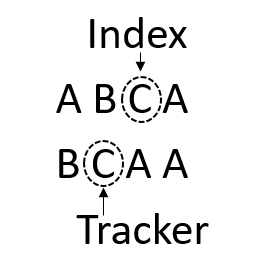
\includegraphics[height=4cm]{include/index-tracker.png}
				\end{center}
				{\footnotesize{Example of the index and tracker}}

		\subsection{Printing Neatly}

			\paragraph{Greedy Solution:} The greedy solution simply prints as many words as possible on a line before going to the next. The solution it gives is not guaranteed to be optimal.
				\seeAlgorithm{10}

			\paragraph{Dynamic Programming:} The dynamic programming approach computes an optimal solution in polynomial time. First, we define extras[$i,j$] to be the number of extra spaces on a line containing words i through j. Using this, we can compute the cost of a line containing the same words:
			\begin{enumerate}
				\item lc[$i,j$] = $\infty$ 			if extras[$i,j$] < 0   (if words do not fit on the line)
				\item lc[$i,j$] = 0    				if $j = n$ and extras[$i,j$] $\geq$ 0   (if it is the last line and the words fit)
				\item lc[$i,j$] = $(\text{extras}[i,j])^3$ 	otherwise
			\end{enumerate}
			Using this, we can compute the optimal arrangement (minimal cost) of words 1..j = c[j] :
			\begin{enumerate}
				\item $c[j] = 0$ if $j = 0$
				\item $c[j] = \min((1\leq i\leq j),(c[i-1] + lc[i,j]))$ if $j>0$
			\end{enumerate}
			\seeAlgorithm{11}

			\paragraph{Recursive:} The recursive solution iterates through all the possible sequences and returns the optimal score and solution.
			\seeAlgorithm{12}

			\paragraph{Branch and Bound:} Two branch and bound methods were compared, in both cases an initial estimate of the upper bound was evaluated using the the cost of a greedy approach. The first method then evaluates solutions in the same manner as the recursive, but when the cost of the current branch exceeds the bound given by the greedy solution, the recusion is cut and the algorithm back-tracks. The second algorithm makes an estimate of the cost of the remaining solution by using a greedy approach to find the cost of any remaining words, this enables to algorithm to cut potentially worse solutions early. The second approach is faster than the dynamic approach but unfortunately does not alway produce an optimal solution.


	\section{Preprocessing techniques}
		\paragraph{Introduction:} We came up with four different preprocessing techniques to aid in detecting plagiarism. Each technique can be implemented on the two input texts and then the LCS is computed on the results of the preprocessing.

		\subsection{Light Preprocessing}
			The most basic preprocessing replaces certain symbols to make the texts more universal. In this technique, directional quotes (quotation marks that indicate if a quote is starting or finishing) are replaced by straight quotes, and extra newline characters and spaces are removed.

		\subsection{Advanced Preprocessing}
			Advanced preprocessing deletes all non-ascii characters and all symbols that are not periods or commas, and makes everything lower case. This is done to make the LCS more robust to small changes in punctuation. For example, the following is an text before preprocessing:
			\corpustext{This kind of relationship can be visualized as a tree structure, where `student' would be the more general root node and both `postgraduate' and `undergraduate' would be more specialized extensions of the `student' node (or the child nodes).}

			And here would be the same text after advance preprocessing:
			\corpustext{this kind of relationship can be visualized as a tree structure, where student would be the more general root node and both postgraduate and undergraduate would be more specialized extensions of the student node or the child nodes.}


			\paragraph{Stop Word Removal:} For stop word removal preprocessing, an input text is run through the advanced preprocessing technique seen above and then passed to a function that deletes all occurrences of stop words. Stop words are any words that do not carry any significance to the similarity of two texts.
			We chose to remove them as a possible preprocessing technique to make the LCS robust to students simply adding in meaningless words to cover plagiarism.
			The stop words are listed in a file. Examples of stop words include ``furthermore'', ``regardless'', and ``somehow''.\\
			Below is the same example sentence from above after stop word removal:
			\corpustext{kind relationship visualized tree structure, student would general root node postgraduate and undergraduate specialized extensions student node child nodes}
			However, we need to take care about the number of stop words we're removing, because by suppressing too much of them, the sentence can be so simple that finding the LCS don't even make sense anymore.

			Stop Word preprocessing delete some `useless' words (according to a certain dictionary), so the running time is improved. But if you remove too many words, the algorithm is useless. So we have to balance it well, so a lot of test were done.


			\paragraph{Word Ordering} Word ordering preprocessing starts by feeding an input text to the advanced preprocessing technique from above. Then, each sentence in the text is reordered so that the words in the sentence are arranged alphabetically. This is done so that texts that have copied and rearranged content from an original text are still detected as plagiarism.\\
			Below is the same original sentence from above, after the word ordering preprocessing:
			\corpustext{a and and as be be be both can child extensions general kind of more more node nodes of or postgraduate relationship root specialized structure, student student the the the this tree undergraduate visualized where would. }


	\section{Graphical User Interface}
		\subsection{Plagiarism detector}
			The Graphical User Interface (GUI) uses a \textsc{Python} library called \texttt{PyQt4}. \\
			In this first tab called `LCS Unit', we have many separated areas splitted as follows:
			\seeFigure{2}
			\begin{enumerate}
				\item on the left: LCS inputs:
				\begin{enumerate}
					\item option bar:
					\begin{itemize}
						\item \tw{Task} : task from the corpus
						\item \tw{Text} : text from the corpus
						\item \tw{LCS preprocess} can be selected among:
						\begin{itemize}
							\item \tw{Raw}
							\item \tw{Advanced preprocessing}
							\item \tw{preprocessing}
							\item \tw{swr (stop words removal) preprocessing}
							\item \tw{WordOrgering preprocessing}
						\end{itemize}
						\item \tw{LCS algorithm} can be selected among:
						\begin{itemize}
							\item \tw{LCS} (classic)
							\item \tw{LCS Sentence} (by sentence)
						\end{itemize}
					\end{itemize}
					\item the text to compute from the corpus
					\item the `wiki' text to compare with
				\end{enumerate}
				\item on the right: LCS results:
				\begin{enumerate}
					\item printing neatly section :
					\begin{itemize}
						\item max-width slider (from 20 to 60)
						\item algorithm chooser (Dynamic or Greedy)
						\item the LCS printed neatly according to the width and the algorithm
					\end{itemize}
					\item some numbers resulted from the computation:
					\begin{itemize}
						\item the original length of the text from the corpus
						\item the LCS length
						\item the plagiarism score, defined as follow : \\
							let $T$ be the original text, and $s_i$ the subsentences of $T$ where words from the LCS are side-by-side in $T$ (words in bold in the GUI). Then we can compute:
							$\text{score} = \sum_{i}(|s_i|)^2$
						\item the actual running time to find the LCS
						\item then, a pie chart showing the percentage of plagiarized text \textit{vs.} the original one.
					\end{itemize}
				\end{enumerate}
			\end{enumerate}
		

		\subsection{Data table}
			We used an \textsc{Excel} file (\tw{corpus-final09.xls}) to store informations concerning the execution of all the algorithms on all the texts from the corpus.
			\seeFigure{3}
			\begin{itemize}
				\item \sqbr{A} the name of the file
				\item \sqbr{B:D} group, person and task
				\item \sqbr{E:F} the category of plagiarism, native or not
				\item \sqbr{G:H} knowledge and difficulty
				\item LCS Length and Ratios for:
				\begin{itemize}
					\item \sqbr{I:J} no preprocessing
					\item \sqbr{K:L} light preprocessing
					\item \sqbr{M:N} advanced preprocessing
					\item \sqbr{O:P} by sentence, advanced preprocessing
					\item \sqbr{Q:X} without stop words (again with no,advanced,light preprocessing, and alphabetical ordering)
				\end{itemize}
			\end{itemize}

		\subsection{Graphs}

			\paragraph{General graph:} In this third tab, we are simply showing the LCS ratios (LCS length over text length) for all the files, and for the different preprocessing techniques. We can see that the more advanced the preprocessing, the longer the LCS: that is exactly what we wanted.
			\seeFigure{4}

			\paragraph{Graph by task:} The fourth tab shows the LCS Ratio for each task (and for each text of the corpus referring to this task), labeling with different colors the plagiarism category given by the \textsc{Excel} file. The labels are confirmed by this graph: we see that the `cut' category as a much higher LCS ratio than the `light' and `heavy' ones, and the `non' are very low.
			\seeFigure{5}

			\paragraph{Repartition by category:} This last tab is here to display the repartition of each LCS ratio over the plagiarism categories (non plagiarized, heavy modified, light modified and cut from the text)
			\seeFigure{6}


	\newpage
	\section{Experimental study}
		\subsection{Time complexity}
			\paragraph{LCS Dynamic Programming:} The dynamic programming algorithm for finding the length of the LCS requires $\bigO(mn)$ time, where m and $n$ are the lengths (number of words) of the two input texts. This can be observed from the algorithm itself, as there is a for loop from 1 to $n$ nested inside a for loop from 1 to $m$. The recursive algorithm used to build the solution from the b matrix requires $\bigO(m+n)$ time. Each run of the algorithm takes constant time, and each recursive call to the algorithm decreases at least one of the lengths by one. Combining these two results gives a time complexity of $\bigO(mn)$ to compute the length and build the LCS.

			\paragraph{LCS Linear Space (Forwards and Backwards):} The linear space versions of the dynamic programming algorithm do the same computations, with an added step at copying the row of the matrix after each row iteration. As a result, the asymptotic time complexity remains $\bigO(mn)$.

			\paragraph{LCS Divide and Conquer:} Let $T(m,n)$ denote the run time of the algorithm. At each call of the algorithm, it performs two $\bigO(mn)$ calls to the space-efficient algorithm. Then it makes two recursive calls on strings of size $q$ and $\frac{n}{2}$, and $m - q$ and $\frac{n}{2}$, respectively. Then, for constant $c$, we have:
				\begin{align*}
					T(m,n) &\leq cmn + T(q,\frac{n}{2}) + T(m-q,\frac{n}{2}) \\
					T(m,2) &\leq cm \\
					T(2,n) &\leq cn
				\end{align*}
			If we assume $m = n$ and $q = \frac{n}{2}$, then we have:
				$$T(m,n) \leq 2T(\frac{n}{2}) + cn^2$$
			From the master theorem, we have $a = 2, b = 2, f(n) = n^2$, and $\log b(a) = 1$.
			Then, since $f(n)$ is $\Omega(n^c)$ where $c=2>\log b(a)=1$, and the regularity condition holds, since $2(\frac{n^2}{4}) \leq kn^2$ with $k = \frac{1}{2}$, then it follows that $T(m,n) = \Theta(f(n)) = \Theta(n^2)$.
			So, when m=n, the run time is $\Theta(n^2)$. We can assume that when $m \neq n, T(m,n) \leq kmn$, and prove it by induction:
			assume $T(m',n') \leq km'n'$ for $m'<m$ and $n'<n$:
			\begin{align*}
				T(m, n) &\leq cmn + T(q,\frac{n}{2}) + T(m-q,\frac{n}{2}) \\
					&\leq cmn + kq(\frac{n}{2}) + k(m-q)(\frac{n}{2}) &&\text{(by induction hypothesis)} \\
					&= cmn + kq(\frac{n}{2}) + km(\frac{n}{2}) - kn(\frac{n}{2}) \\
					&= (c+k/2)mn.
			\end{align*}
			So, if $c = k/2$, then the proof works. Thus, the LCS divide and conquer has a time complexity of $\bigO(mn)$

			\paragraph{LCS Recursive:} The recursion for the recursive solution is as follows:
			\begin{align*}
				T(m,n) &= T(n,m-1) + T(n-1,m) + c \\
					&= (T(n,m-2) + T(n-1,m-1) + T(n-1,m-1) + T(n-2,m)) + c' \\
					&\geq 2T(n-1,m-1)
			\end{align*}
			Therefore the algorithm is exponential, since it is $\bigO(2^{\min(n,m)})$

			\paragraph{LCS Branch and Bound:} In the worst case, the branch and bound solution take the same time as the recursive. Thus, it is exponential. However, in practice, it is faster (see runtimes).

			\paragraph{Printing Neatly Greedy Solution:} In the greedy algorithm, there is just one iteration over the whole text, as a decision is made to print a word on the same line if possible or move to the next line. As a result, the time complexity is $\bigO(n)$ where $n$ is the number of words in the text.

			\paragraph{Printing Neatly Dynamic Programming:} The dynamic programming algorithm can be broken into 3 sections: first, computing the extras matrix; next, computing the line cost matrix; and finally, computing the optimal solution.
			\begin{enumerate}
				\item The extras matrix is an $n \times n$ matrix where each element is computed in constant time. Thus, it is $\bigO(n^2)$.
				\item The line cost matrix is also an $n \times n$ matrix with constant cost for each element, so it is $\bigO(n^2)$.
				\item The optimal cost matrix is an array of length n, but the cost to compute the element at index $i$ is a function of $i$. Thus, it is $\bigO(n^2)$.
			\end{enumerate}
			Since all three main parts of the algorithm are $\bigO(n^2)$, the algorithm is $\bigO(n^2)$.

			\paragraph{Printing Neatly Recursive:} The recursive solution iterates through all possible solutions of lines that have at least one word on each line and have 0 or more spaces on the end (that fit). Let $i$ be the number of words that can fit on the first line, then we have the following recursion:
				$$T(n) = T(n-1) + T(n-2) + \cdots + T(n-i)$$
			Expanding each recursion on the right hand side of the equation gives an exponential growth.

			\paragraph{Printing Neatly Branch and Bound:} In the worst case, the branch and bound extension behaves just as the plain recursive algorithm, thus it is also exponential. However, the bounding can limit the number of unneeded computations (see runtimes).



		\subsection{Runtime analysis}
			\subsubsection{LCS}
				We have run the different algorithms (Branch \& Bound, Recursive, Divide \& Conquer and Dynamic) with a different number of words, to study their time complexity. Then, we plotted this data into three different graphs, in the goal to better see what happens.

				\paragraph{Running times on linear scale / $|\text{words}|$:} in this graph, the two scales are linear, and we can already observe the speed of each algorithms, and say that the Branch \& Bound and the Recursive are much slower than the Divide \& Conquer and the Dynamic algorithms.
				\seeFigure{8}
				
				\paragraph{Running times on logarithmic scale / $|\text{words}|$:} The have a better view of the complexity of the slower algorithms, we draw the same graph, but changing the time scale from linear to logarithmic. Now, we see that the Branch \& Bound and the Recursive are linear in this scale, then we can deduce that, graphically, this two algorithms should be exponential.
				\seeFigure{9}
				
				\paragraph{Running times on logarithmic scale / $(|\text{words}|)^2$:} This time, we keep the time scale linear, but the $x$-axis becomes the number of words \textbf{squared}. We demonstrate that the running time of the dynamic algorithms is far more efficient than the recursive and branch and bounds methods, and the time complexity is quadratic in $n$ (where $m = n$)
				\seeFigure{10}

			\subsubsection{Printing Neatly}
				\paragraph{Running times on linear scale / $|\text{words}|$:} Here we see that the more efficient algorithm to print neatly is the Greedy one, and the less efficient is the Recursive one.
				\seeFigure{11}
				
				\paragraph{Running times on logarithmic scale / $|\text{words}|$:} Now, the Branch \& Bound and the Dynamic algorithms are close from each other, and the Dynamic one is slightly worse.
				\seeFigure{12}

				\paragraph{Running times on linear scale / $(|\text{words}|)^2$:}
				\seeFigure{13}




		\subsection{Space complexity}
			\paragraph{LCS Dynamic Programming :} In the dynamic programming algorithm, there are two $m \times n$ matrices ($m$ is length of first input text, $n$ is length of second), one for the $c$ matrix denoting optimal solutions, and one for the $b$ matrix that is used to build the solution. These matrices are in addition to the two input word arrays and LCS word array. Thus, the space complexity is $\bigO(mn)$.

			\paragraph{LCS Linear Space (forward and backward):} In the linear space versions of the dynamic programming algorithm, we don't use the $b$ matrix, and the $c$ matrix is reduced to just 2 rows by $n$ columns. Thus, the space complexity is $\bigO(n)$.

			\paragraph{LCS Divide and Conquer:} The divide and conquer algorithm uses the linear space algorithm on each half of the first input text and the full second text. The space complexity for these algorithms alone is $\bigO(n)$; however, we must save the full column indexed at $j = \frac{n}{2}$ in order to find the optimal row to divide our problem. Since there are m rows, the space needed to save the two columns (one for forwards LCS, one for backwards LCS) is $2m$. Adding this to the $\bigO(n)$ from the linear space algorithm, we have a space complexity of $\bigO(m+n)$.

			\paragraph{LCS Recursive:} Since the algorithm does a depth first search of the search space, a search will go all the way to a leaf node (base case) before backtracking back up the call tree. Each call to the function needs the two input texts that get smaller as the search gets closer to the base case. In terms of space used in addition to the input texts, the space complexity is constant. However, if a new copy of each input text is made for each recursive call, the space complexity becomes $\bigO(n^2 + m^2)$ in the worst case, which is when a leaf node is found in the search space and both input texts have been reduced to a length of 2 or less:
			\begin{align*}
				S(m,n) &= (m+(m-1)+...+1) + (n+(n-1)+...+1) \\
					&= \frac{(m^2 + m)}{2}  + \frac{(n^2 + n)}{2} \\
					&= \bigO(m^2) + \bigO(n^2) \\
					&= \bigO(m^2 + n^2)
			\end{align*}
			However, if pointers are used and new copies of the input texts are not made for each recursive call, then the space complexity become linear with respect to the input texts lengths.

			\paragraph{LCS Branch and Bound:} The space complexity for the the branch and bound extension is the same as recursive algorithm, except that a Queue of possible solutions to explore is also kept, which could potentially get quite large.


			\paragraph{Printing Neatly Greedy:} There are no additional matrices or arrays used to compute the greedy solution, as the input text is the only array stored. Thus, the space needed is linear, $\bigO(n)$ where $n$ is the number of words in the input text.

			\paragraph{Printing Neatly Dynamic Programming:} The dynamic programming algorithm uses two matrices (one for extras, one for line cost) of size $n \times n$, where $n$ is the number of words in the input text. Additionally, an array of size $n$ is used to compute the optimal solution. Thus, the asymptotic space complexity is $\bigO(n^2)$.

			\paragraph{Printing Neatly Recursive:} There are no additional matrices or arrays used for the plain recursive solution. Thus, as long as pointers are used instead of copying a new input text array for each recursive call, the space complexity is $\bigO(n)$. If copies are made, then the space complexity would be $\bigO(n^2)$ (see LCS recursive space complexity analysis).

			\paragraph{Printing Neatly Branch and Bound:} The space complexity is that of the recursive solution plus an array of possible solutions to explore. This array is created at each level of recursion, and contains at most every word in the input. Since there are at most $n-1$ levels of recursion (in the case where there is just one word per line), the worst case space complexity would be $\bigO(n^2)$.

		\subsection{Outliers}
			If we look again at the Figure 5: Graph by task, we can see that there is three `cut' texts that have a LCS ratio less than 70\% (in task b and c). After looking each files (for example \texttt{g4pD\_taskb.txt} with \texttt{orig\_taskb.txt}), we concluded that this is an error by the original classification which was given to us.

		\subsection{Scalability}
			\paragraph{LCS:} For input texts that are very large, it is clear that the LCS Divide and Conquer strategy would scale the best out of all of them. It runs in pseudo-polynomial time which is much faster than the recursive or branch and bound solutions. Also, the space improvement over the classic dynamic programming algorithm would be needed when the input texts are very large.

			\paragraph{Printing Neatly:} If an input text is very large, the recursive and branch and bound solutions would take too long. Furthermore, since the dynamic programming approach takes polynomial space and time, it would be unsuitable for extremely large input texts. The only solution left is the greedy solution, which takes linear space and time. It offers the best chance of scaling reasonably with large input texts. However, the solution is not guaranteed to be optimal. If an optimal solution was needed, the dynamic programming algorithm would offer the best scalability.

	\section{Plagiarism Detector}
	
Several techniques and methods were explored in order to find the most suitable method of evaluating whether a text is plagiarised or not. Initial attempts were based of a ratio between size of the corpus text and the size of the LCS text, but these were found to be error prone and susceptible to misclassification due to the number of stop words in the texts. Removing the stop words did improve this, but did not take into account how group together words were in the provided text. Our final method of detecting plagiarism uses the LCS that was found between two texts, and combines two types of comparisons between the LCS and the text in question to determine if the text was plagiarized or not.

First, we compute how many words in the LCS appear next to each other in the original text. This is done 
because texts that are copied are more likely to have copied words next to each other, as opposed to texts 
that aren't copied and just have similar words. Our function computes the square of the number of words 
that are adjacent to each other (one word alone is 1, two words next to each other would be 4), divides this 
number of by the square of the length of the text to obtain a ratio (a ratio of 1 would mean cut and paste)
and then returns the square root of this number.

Second, we compute the ratio of sentences in the text that have a percentage of plagiarism higher than a 
certain threshold. This threshold is an argument to the function and can change. We have found that an optimal 
threshold is 70\%, meaning this function returns the ratio of sentences in the text that are more than 70\% 
plagiarized. However, the user can change the threshold depending on how much time they have to check a text,
for example. A lower threshold will result in higher plagiarism scores, and more texts to examine for potential 
plagiarism. 

Finally, we combine these two results to form the suggestion on if the text is plagiarized or not. First, we compute 
a combined threshold for the sum of both metrics. We have found through experimentation that all the texts in the 
corpus that are not plagiarized have combined scores of less than 0.2 out of 1. Thus, we set our threshold sum as 0.2. 
\seeFigure{14}
Next, we compute the combined plagiarism score for a text by adding the first metric to the second.
We then return whether or not this combined score is higher than the combined score threshold.
	
	\section{Project planning \& difficulties}
		\paragraph{Planning:}
		In general the project went mostly to plan, but there were a few notable changes to the deadlines. The initial plan did not contain either the LCS recursive or the LCS space efficient algorithms. The LCS dynamic backwards took longer than was expected to implement, in order to stay on schedule, another team-member worked on the LCS branch and bound algorithm. The user interface was continually improved beyond the its original dead, as team-members had new ideas of features that could be incorporated into its design. The more advanced pre-processing was done earlier on than planned. Finalised the technique for plagiarism took longer than expected which meant there were delays to both the start of the report and the presentation.

		\paragraph{Difficulties:} The main goal of coding the LCS algorithm was to implement what we saw during the course.\\
  A hard aspect of the project was translating the pseudo-code into an implementation in Python. It required us to really understand what every part of algorithm was doing, as we had to implement the lower level tasks not included in the slides.\\
  One example of a problem we ran into using Python to implement our algorithms was that Python is zero-indexed, so the first element in a list is indexed at 0. This was a problem because all the algorithms were implemented in the slides using one-indexed pseudo-code. We overcame this by having an empty element in the beginning of every list, to make them line up. Another difficulty we had was combining all of our work into one product. This was not a huge problem, but it did take some time to get all the functions working together in different parts of the software.\\
  Lastly, it was difficult to create preprocessing techniques for the input texts. Our goal was to make the LCS of the preprocessed texts more correlated to the amount of plagiarism. We noticed that some of the corpus texts that were marked as highly plagiarized had short LCS. Thus, we investigated possible reasons for this happening and tried to augment the input texts to make the LCS more revealing. This required a lot of brainstorming and experimenting, as we had to try a lot of different things and collect a lot of data. It turned out to be one of the more time-consuming aspects of the project.

	\newpage
	\section{Conclusion}

		To achieve the goals set out for this project we decided to split it in different parts for each member of the group. Some had to implement LCS algorithms, others the printing neatly algorithm, some of us worked on the space and time complexity analysis, and finally some on the UI. The precise schedule ensured that we achieved what initially set out to do. Even if small changes were made to it, we tried as much as possible to adhere to the original one to in order to stay on track for the final deadline.
To conclude we managed to implement all the LCS algorithms (Classic Forwards and backwards, Linear Space Forwards and Backwards, Divide and Conquer, Recursive and Branch and Bound), and all the Printing Neatly Algorithms, we were able to create a complete and user friendly UI, create different kinds of pre-processing and experiment with and develop techniques for the plagiarism score. Thanks to all of this work, we were able to compare and study them, to improve them and to know which one is the most efficient to use in practice and for our UI.
  To sum up every member of our group were very involved in the project. For some of us the language \textsc{Python} was unknown, and this gave many of us the opportunity to learn a new language or expand our knowledge of \textsc{Python}. \\
  All of the project team are satisfied with the level of cooperation within the group and the final result that has been achieved.

\section{References}

[1] Gaofeng Huang and Andrew Lim.   \textit{An Effective Branch-and-Bound Algorithm to Solve the
k-Longest Common Subsequence Problem}




% \appendix
\newpage

	\section*{Appendices}
	
	\addcontentsline{toc}{section}{Appendices}
	\listofalgorithms
	\listoffigures

	\newpage
		\algo{ % 1
			\caption{Optimal substructure}
			\KwData{texts $X,Y$ with lengths $m,n$}
			\For{an LCS $Z = <z_1,\cdots,z_n>$}{
				\If{$X_m = Y_n$}{
					$X_m = Y_n = z_k$\;
					$z_{k-1}$ is the LCS of $X_{m-1}$ and $Y_{n-1}$\;
				}
			}
			\uIf{$X_m \neq Y_n$}{
				$z_k \neq X_m \Rightarrow Z$ is the LCS of $X_{m-1}$ and $Y_n$\;
			}\If{$X_m \neq Y_n$} {
				$z_k \neq Y_n \Rightarrow Z$ is the LCS of $X_m$ and $Y_{n-1}$\;
			}
		}

		\algo{ % 2
			\caption{Recursive solution}
			\KwData{texts $X,Y$ with lengths $m,n$}
			\uIf{$i = 0$ or $j = 0$}{$c[i,j] = 0$\;}
			\uIf{$i,j > 0$ and $X_i = Y_j$}{$c[i,j] = c[i-1,j-1] + 1$\;}
			\If{$i,j > 0$ and $xi \neq yj$}{$c[i,j] = \max(c[i-1,j],c[i,j-1])$}
		}

		\algo{ % 3
			\caption{LCS-Length(input: $X,Y$)}
			% \KwData{texts $X,Y$ with lengths $m,n$}
			$m$ = $|X|$\;
			$n$ = $|Y|$\;
			$b[1..m,1..n], c[0..m,0..n]$\;
			\lFor{$i \in 1..m$}{$c[i,0] = 0$}
			\lFor{$j \in 0..n$}{$c[0,j] = 0$}
			\For{$i \in 1..m$}{
				\For{$j \in 1..n$}{
					\uIf{$xi = yj$} {
						$c[i,j] = c[i-1,j-1] + 1$\;
						$b[i,j] = 'd'$ \CommentSty{\#for diagonal}\;
					}\uElseIf{$c[i-1,j] \geq c[i,j-1]$}{
						$c[i,j] = c[i-1,j]$\;
						$b[i,j] = 'u'$ \CommentSty{\#for up}\;
					}\Else{
						$c[i,j] = c[i,j-1]$\;
						$b[i,j] = 'l'$ \CommentSty{\#for left}\;
					}
				}
			}
			\Return{$c$ and $b$}
		}

		\algo{ % 4
			\caption{Print-LCS(input: $b, X, |X|, |Y|)$}
			\uIf{$i = 0$ or $j = 0$}{
				return\;
			}\uIf{$b[i,j] = `d'$}{
				Print-LCS($b,X,i-1,j-1$)
			}\uElseIf{$b[i,j] = `u'$}{
				Print-LCS($b,X,i-1,j$)
			}\Else{
				Print-LCS($b,X,i,j-1$)
			}
		}

		\algo{ % 5
			\caption{LCS\_LSF (input: $X,Y$)}
			$m = |X|$\;
			$n = |Y|$\;
			$c[1..2,1..n]$\;
			$\text{col} = []$ \CommentSty{\#for use in divide and conquer alg (see next section)}\;
			\For{$i \in 1..m$}{
				$c[1,0] = 0$\;
				\For{$j \in 1..n$}{
					\uIf{$xi = yj$}{$c[1,j] = c[0,j-1] + 1$\;}
					\uElseIf{$c[1,j-1] > c[0,j]$}{$c[1,j] = c[1,j-1]$\;}
					\Else{$c[1,j] = c[0,j]$\;}
				}
				$c[0,:] = c[1,:]$\;
				$\text{col.append}(c[1,n])$\;
			}
			\Return{$c[1,length_Y],$col} \CommentSty{\#return length of LCS, column}
		}

		\algo{ % 6
			\caption{LCS\_LSB(input: $X,Y$)}
			$m = |X|$\;
			$n = |Y|$\;
			$c[1..2,1..n]$\;
			$\text{col} = []$ \CommentSty{\#for use in divide and conquer alg (see next section)}\;
			\For{$i \in m-1..0$}{
				\For{$j \in n-1..0$}{
					\uIf{$X[i+1]=Y[j+1]$}{$c[1,j] = c[0,j+1]+1$\;}
					\uElseIf{$c[1,j+1]>c[0,j]$}{$c[1,j] = c[1,j+1]$\;}
					\Else{$c[1,j] = c[0,j]$\;}
				}
				$c[0,:] = c[1,:]$\;
				$\text{col.insert}(0,c[1,0])$\;
			}
			\Return{$c[1,0], \text{col}$} \CommentSty{\#length of LCS, column}
		}

		\algo{ % 7
			\caption{LCS\_DC(input: $X,Y$)}
			$m = |X|$\;
			$n = |Y|$\;
			\If{$m*n = 0$}{
				\Return{$[]$} \CommentSty{\#if one of the texts is empty, return an empty LCS}
			}\ElseIf{$m \leq 2 \text{ or } n \leq 2$}{
				\Return{LCS\_DyProg(X,Y)} \CommentSty{\#if one of the texts is small, can do normal Dynamic Prog}
			} \Else{
				$\text{breakpt} = \text{floor}(n / 2)$\;
				$\text{length}, c = \text{LCS\_LSF}(X, Y[0:\text{breakpt}])$\;
				$\text{length2}, c2 = \text{LCSLSB}(X, Y[\text{breakpt}:n])$\;
				$q = \text{maxindex}(c, c2)$ \CommentSty{\#q is the index that maximizes ($c[q] + c2[q]$)}\;
				$\text{LCSL} = \text{LCS\_DC}(X[0..q],Y[0..\text{breakpt}])$\;
				$\text{LCSR} = \text{LCS\_DC}(X[q+1,m],Y[\text{breakpt}+1,n])$\;
				\Return{$\text{LCSL} + \text{LCSR}$}  \CommentSty{\#return concatenation of sub LCS}
			}
		}

		\algo{ % 8
			\caption{LCS\_Recursive(input: $X, Y$)}
			$m = |X|$\;
			$n = |Y|$\;
			\If{$X[m] = Y[n]$}{
				\Return{LCS\_Recursive($X[0:m-1], Y[0:n-1]$)}\;
			} \Else{
				LCS1 = LCS\_Recursive($X[0:m-1], Y[0:n]$)\;
				LCS2 = LCS\_Recursive($X[0:m], Y[0:n-1]$)\;
				\lIf{$|LCS1| > |LCS2|$}{
					\Return{LCS1}
				} \lElse{
			 		\Return{LCS2}
			 	}
			}
		}

		\algo{ % 9
			\caption{Brand\_and\_bound(inputs: $X,Y$)}
			max\_lcs\_length = min($X$.length, $Y$.length)\;
			best = find\_lower\_bound($X,Y$) – 1\;
			starting\_solution = (1 $<<$ max\_lcs\_length) – 1\;
			best\_solution =  0\;
			index = -1\;
			tracker = -1\;
			LIFO\_queue.put([starting\_solution, index, tracker, best])\;

			\While{LIFO\_queue is not empty}{
				node = LIFO\_queue.get()\;
				\uIf{node.index = max\_lcs\_length and node.best $>$ best}{
					best = node.best\;
					best\_solution = node.solution\;
				}\Else{
					\If{node.bound $>$ best}{
						child1 = node.child1
						child2 = node.child2
					}
					\If{find\_upper\_bound(child1) $>$  find\_upper\_bound(child2)}{
						\lIf{child2.bound $>$ best}{LIFO\_queue.add(child2)}
						\lIf{child1.bound $>$ best}{LIFO\_queue.add(child1)}
					}\Else{
						\lIf{child1.bound $>$ best}{LIFO\_queue.add(child1)}
						\lIf{child2.bound $>$ best}{LIFO\_queue.add(child2)}
					}
				}
			}
			\Return{best\_solution}\;
		}

		\algo{ % 10
			\caption{PN\_Greedy(input: X (list of words to be printed), L (number of spaces per line))}
			lines = []\;
			currentLine = []\;
			currentLineSpace = 0\;
			\For{$i$ in $X$}{
				\If{currentLineSpace + $(|X[i]| + 1) \leq L$}{
					currentLineSpace += $|X[i]| + 1$   \CommentSty{\#update space taken on current line (for space between words)}\;
					currentLine += " " + $X[i]$\;
				}\Else{
						lines.append(currentLine)\;
						currentLineSpace = $|X[i]|$\;
						currentLine = $X[i]$\;
				}
			}
			lines.append(currentLine)\;
			\Return{lines}\;
		}

		\algo{ % 11
			\caption{PN\_DP(input: $X, L$)}
			Compute extras[$i, j$],$ 1 = i, j = n$\;
			Compute lc[$i, j$],$ 1 = i, j = n$\;
			$c[0] = 0$\;
			\For{$j \in 1..n$}{
				$c[j] = \min((1\leq i\leq j),(c[i-1] + lc[i,j])) $\;
				$p[j] = k \text{ s.t. } \min(1\leq i\leq j)(c[i-1] + lc[i,j]) = c[k-1] + lc[k,j]$ \CommentSty{\#store where the cuts are}\;
			}
			\Return{$p$}
		}

		\algo{ % 12
			\caption{PN\_Recursive(input: $X, L$)}
			result = [] \CommentSty{\#where the lines will be stored}\;
			max\_words = the maximum number of words that can fit on current line \CommentSty{\#what the greedy solution would return}\;
			\If{max\_words $\geq |X|$}{
				\Return{$0, X[0:|X|]$} \CommentSty{\#base case: where all words inputed will fit on current line}\;
			}
			best\_score = $\infty$\;
			\For{$i \in 1..\text{max\_words}$}{
				subscore = 0 \CommentSty{\#current line space taken}\;
				\For{$j \in 0..i-1$}{
					subscore += $|X[j]| + 1$ \CommentSty{\#add current word and space}\;
				}
			 	subscore -= 1 \CommentSty{\#remove last space}\;
			 	subscore = $(L - \text{subscore})^3$ \CommentSty{\#compute cost of space left over}\;
				score, res = PN\_Recursive($X[i:n], L$)\;
			 	\If{score + subscore < best\_score}{
			 		result.append($X[0..i]$)\;
					result += res\;
				}
			}
			\Return{best\_score, result}
		}


		\screenshotWithComment{Path to the solution of the LCS of [A,B,C,A] and [B,C,A,A]}{branch-and-bound.png}{The path explored first shown as a dashed line, the super-script numbers at the top right show the score and upper bounds computed at each stage.}

		\screenshot{LCS Unit}{tab1.png}
		\screenshot{Table}{tab2.png}
		\screenshot{General graph}{tab3.png}
		\screenshot{Graph by task}{tab4.png}
		\screenshot{Repartition by Category}{tab5.png}
		
		\screenshot{Normal distributions of the repartition by category / $|\text{words}|$}{normal.png}

		\screenshot{Running times for different algorithms on linear scale / $|\text{words}|$}{time1.png}
		\screenshot{Running times for different algorithms on logarithmic scale / $|\text{words}|$}{time2.png}
		\screenshot{Running times for different algorithms on logarithmic scale / $(|\text{words}|)^2$}{time3.png}

		\screenshot{Comparison between Printing neatly algorithms, linear scale.}{time4.png}
		\screenshot{Comparison between Printing neatly algorithms with a log score, showing the exponential runtimes of the recursive and branch and bound (optimal) algorithms.}{time5.png}
		\screenshot{Comparison between the Printing neatly Dynamic, Branch \& Bound (non-optimal) and greedy algorithms}{time6.png}
		\screenshot{The final scores of the plagiarism detector. Excluding outliers, a good separation is observed between the non-plagiarised texts (yellow).}{plagiarism_scores.png}

		\screenshot{Planning: the plan at the start of the project.}{planning1.png}
		\screenshot{Planning: the actual dates.}{planning2.png}





\end{document}
